\chapter{Theoretische Grundlagen}

\section{Stabilität in Inselnetzen}

\section{Speichertechnologien in Inselnetzen}

\subsection{Gründe für den Einsatz von Speichern in Inselnetzen}
Für diese Projektarbeit soll ein autarkes Inselnetz mit regenerativer Energieeerzeugung 
modelliert und simuliert werden.
Aus verschiedenen Gründen, welche im Folgenden genauer erläutert werden sollen, ist der Einsatz von
Speichertechnologien für die Umsetzung eines solchen Inselnetzes zwingend notwendig.

Grundlegend ist eine lückenlose Energieversorgung innerhalb eines Netzes nur möglich wenn nahezu gleich viel Energie in das Netz
eingespeist und abgenommen wird.
Entscheidende Parameter für die Regelung der Energieerzeugung sind dabei vor Allem die Netzfrequenz 
und -spannung.
Das deutsche Verbundnetz ist dafür in vier Regelzonen unterteilt, welche widerrum in verschiedene
Bilanzkreise unterteilt sind.
Innerhalb dieser Bilanzkreise wird anhand von Vorraussagen für den nächsten Tag versucht
eingespeiste und entnommene Leistung auszuregeln.
Durch den schwankenden Leistungsbedarf sind Abweichungen hier allerdings die Regel.
Bei der Betrachtung eines regenerativen Inselnetzes kommt die volatile Natur von regenerativen Energieerzeugern
als weiterer Faktor hinzu und erschwert eine korrekte Vorraussage enorm.
Diese Abweichungen der tatsächlich benötigten Leistung von der bereitgestellten führen zu Frequenzschwankungen
welche sich wiederrum negativ auf die Netzstabilität auswirken.
Zum Ausgleich dieser Schwankungen muss Regelernegie zur Verfügung gestellt werden.

\begin{figure}[h!]
    \centering
    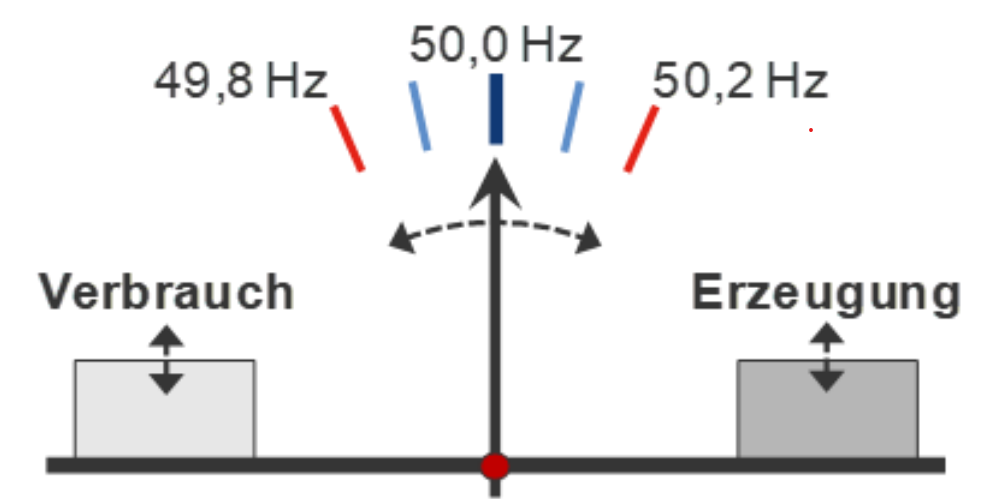
\includegraphics[width=6cm]{Abbildungen/Sollfrequenz.png}
    \caption{Frequenzschwankungen durch Ungleichgewicht von erzeugter und verbrauchter Leistung~\parencite{cronenberg_beschreibung_nodate}}\label{Gleichgewicht}
\end{figure}

Die benötigte Energie ist dabei unterteilt in Momentanreserve, Primärreserve, Sekundärreserve 
und Tertiärreserve.
Die Momentanreserve, welche geringe Frequenzabweichung direkt ausgleichen soll, wird im deutschen Verbundnetz
durch die Schwungmasse der Kraftwerks-Synchronmaschinen bereit gestellt.
Die Primärreserve hingegen greift erst ab einer Abweichung von $20\ mHz$ und musss nach spätestens 30 Sekunden
sowie für mindestens 15 Minuten vollständig zur Verfügung stehen.
Hierfür werden heute schon zunehmend Batteriespeicher eingesetzt.
Zusätzlich wird nach 30 Sekunden die Sekundärregelleistung bereit gestellt, welche für eine Stunde verfügbar sein muss.
Nach 15 Minuten wird diese dann von der Tertiärregelreserve abgelöst, welche ebenfalls fürr eine Stunde verfügbar sein muss.
Die beiden letzten Regeleneergie-Kategorien werden in aller Regel von Kraftwerken in Teillast oder Kraftwerken mit kurzen Anfahrzeiten
erzeugt.
Zuletzt werden einzelne Netzabschnitte vom Netz getrennt um einen Zusammenbruch des Bilanzkreises zu vermeiden.
Dieses Vorgehen bleibt allerdings die äußerste Maßnahme und soll in aller Regel vermieden werden.

Für ein Inselnetz besteht nicht die Möglichkeit Teilnetze abzutrennen. 
Im schlimmsten Fall müssen einzelne Verbraucher und Erzeuger vom Netz getrennt werden um einen stabilen Betrieb zu sichern.
Um das weitestgehend zu vermeiden, ist eine Überdimensionierung von Erzeugern und Speichern meist das Mittel der Wahl.
Große Speicher zur Primärreserve bilden dabei einen wichtigen Grundpfeiler, wobei gerade Batteriespeicher 
auf Grund ihres schnellen Regelverhaltens in Frage kommen~\parencite{Itschner}.

Zusätzlich sollen hier neben der klassischen Regelreserve der Vollständigkeit halber die Regelleistungsprodukte \texttt{Enhanced Frequency Response}
(EFR) und \texttt{Virtuelle Schwungmasse} (VSM) erwähnt werden.
Diese sind zwar noch nicht in den deutschen Markt integriert, könnten aber in der Zukunft eine wichtige Rolle spielen.

EFR setzt dabei schon vor der Primärreserve ein und stellt die volle Regelenergie ab spätestens 1 Sekunde bereit.
Damit füllt EFR die Lücke die durch die fehlenden großen Synchronmaschinen entsteht und wird z.B. bereits vom 
größten britischen Netzbetreiber eingesetzt.
Durch die hohen Anforderungen an die Einschaltzeiten bieten sich auch für diesen Einsatz vor allem
Lithium-Ionen-Batterien an~\parencite{mantar_gundogdu_battery_2018}.

Beim Prinzip der VSM wird versucht die Frequenzstabilität zu verbessern indem Speicher an das Netz angeschlossen werden
die im Wesentlichen das Trägheitsverhalten von mechanischen Schwungmassen in Generatoren imitieren.
Gerade kleiner Inselnetzen welche vor allem durch regenrative Energien betrieben werden könnten hierdurch profitieren.
Auf Grund des kontinuierlichen Energieaustausches mit dem Netz bieten sich für die Umsetzung von VSM-Anlagen vor allem
Speicher mit hoher Lebensdauer und Zyklenzahl an~\parencite{boxleitner_virtuelle_2009}.

\subsection{Rahmenbedingung und Bestimmungen}

In Deutschland sind die Übertragungsnetzbetreiber dafür verantwortlich die Frequenz innerhalb ihrer Regelzone auf möglichst
50 Hz zuhalten.
Dafür stehen Ihnen die oben genannten Regelreserveprodukte zur Verfügung, welche von unterschiedlichen Teilnehmern
des Regelreservemartkes bereit gestellt werden können.
Die verschiedenen Übertragungsnetzbetreiber kooperieren dabei im Netzregelverbund, welcher ein Konzept darstellt,
die Vorhaltung von Regelreserve technisch und wirtschaftlich zu optimieren.
In Zukunft ist ein solches, stark koordiniertes Vorgehen auch auf zentraleuropäischer Ebene geplant.

Im Folgenden sollen die Anforderungen und Bestimmungen zu den einzelnen in Deutschland zugelassenen Regelreserveprodukten 
zusammengefasst werden.

\begin{itemize}
    \item Primärreserve oder \texttt{Frequency Containment Reserve} (FCR) ist darauf ausgelegt die Netzfrequenz möglichst schnell zu stabilisieren. Dafür wird die FCR proportional zur Abweichung der Frequenz von ihrem Sollwert geregelt. Sie wird automatisch bei Abweichungen über 10 mHz aktiviert und soll spätestens nach 30 Sekunden vollständig zur Verfügung stehen.
    \item Sekundärreserve oder \texttt{automatic Frequency Restoration Reserves} (aFRR) löst die Primärreserve ab indem sie die Frequenzabweichung vollständig ausgleicht. Die aFRR ist dafür als Proportional-Integral-Regelung umgesetzt und ist nicht nur abhängig von der Netzfrequenzabweichung sondern zusätzlich vom Leistungsaustausch zwischen den Bilanzkreisen.
    \item Tertiärreserve oder \texttt{manual Frequency Restoration Reserve} (mFRR) löst die aFRR bei länger anhaltenden Störungen ab. Sie ist daher nicht automatisch aktiviert und muss erst innerhalb von 15 Minuten vollständig aktivierbar sein.
\end{itemize}

\begin{figure}[h!]
    \centering
    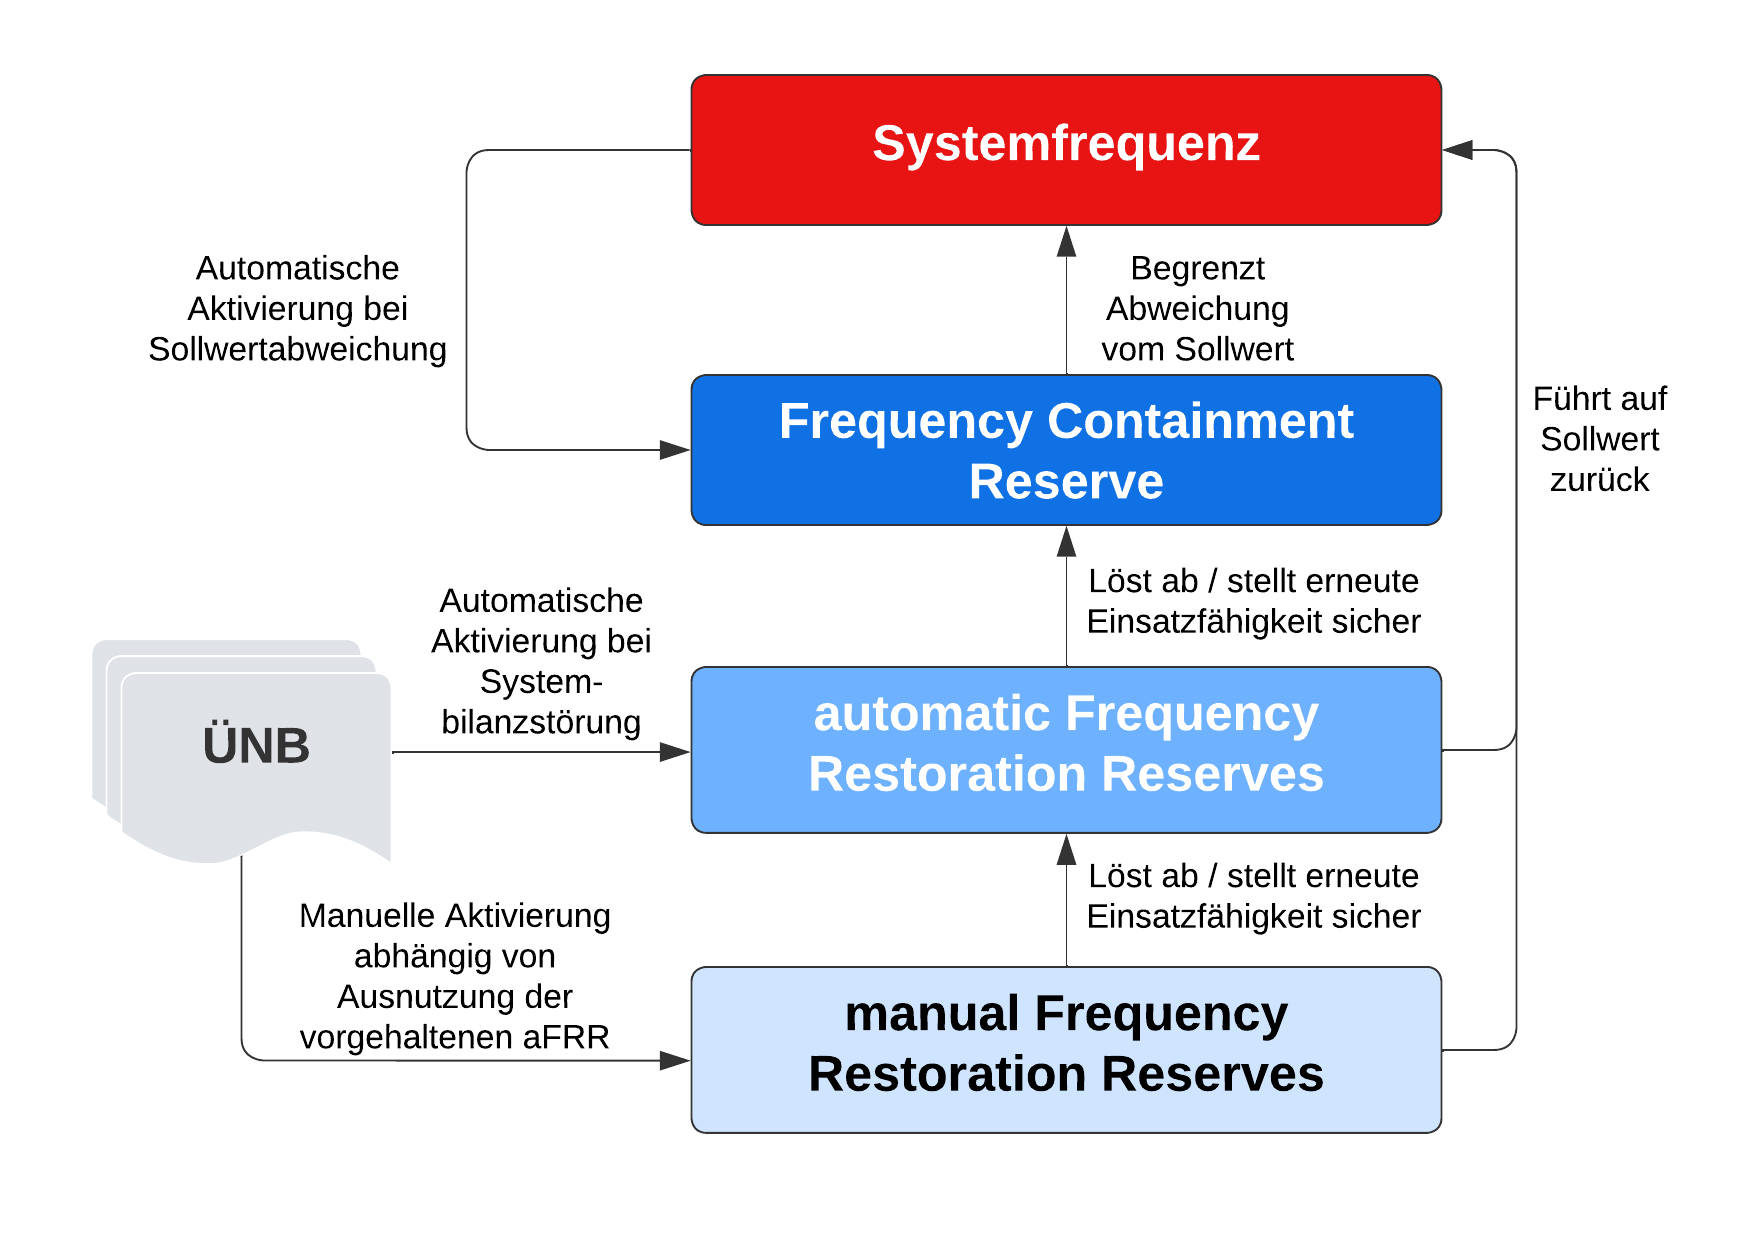
\includegraphics[width=11cm]{Abbildungen/_Flussdiagramm (1).png}
    \caption{Überblick über die verschiedenen Regelreserveprodukte aus~\parencite{cronenberg_beschreibung_nodate}}\label{Fluss}
\end{figure}

\subsection{Betriebsstrategien zu Batteriespeichern}\label{Betriebsstrategien}

Für die Modelle und Simulationen in dieser Projektarbeit werden von den, im letzten Paragraphen beschriebenen Regelreserveprodukten
im Wesentlich zwei genauer betrachtet.
Einerseits die Primärreserve oder FCR und andererseits die EFR, die zwar bisher von deutschen Übertragungsnetzbetreibern nicht genutzt wird
aber gerade für ein Inselnetz wie das hier geplante, eindeutige Vorteile bietet.

Betrachtet man die Anforderungen an diese beide Methoden der Regelleistungsbereitstellung, so kommen vor allem
Batteriespeicher und insbesondere Lithium-Ionen-Batterien für eine Auswahl der Speichertechnologien in Frage.
Im Folgenden sollen verschiedene Methoden zur Umsetzung von FCR- und EFR-Speichern mit Hilfe von Batteriespeichern 
diskutiert und vorgestellt werden.

Beim Betrieb von Batteriespeichern zur Bereistellung von Regelleistung ist der limitierende Faktor der Kapazitäten zu bedenken.
Durch den so genannten State of Charge (SOC) kann ausgedrückt werden, wie viel Prozent ihrer Kapazität einer Batterie noch zur Verfügung stehen.
Um möglichst zu jedem Zeitpunkt die Anforderungen an die PCR oder EFR erfüllen zu können ist eine intelligente
SOC-Steuerung daher unerlässlich.

\begin{figure}[h!]
    \centering
    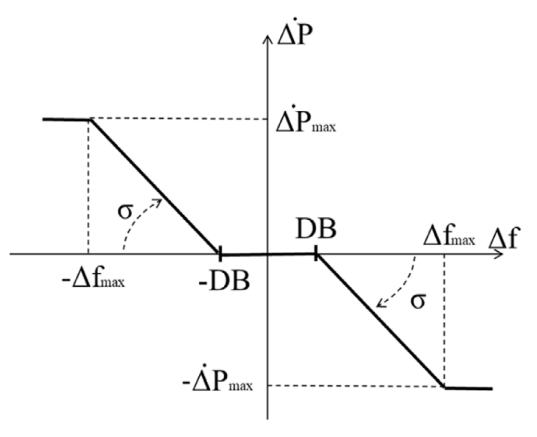
\includegraphics[width=8cm]{Abbildungen/DroopControl.png}
    \caption{Vorgabe der Leistungskurve für PCR-Bereitstellung aus~\parencite[Kap. 3]{noauthor_soc_nodate}}\label{Droop}
\end{figure}

Abbildung~\ref{Droop} zeigt den vorgegebenen Verlauf der Leistungsbereitstellung für PCR-Produkte.
Im letzten Paragraphen wurde bereits beschrieben, dass hierbei ein proportionaler Verlauf zur Frequenzabweichung 
gefordert ist, sobald die Abweichung einen gewissen Grenzwert überschreitet.
Bei einer reinen Umsetzung dieser Kurve mit Hilfe von Batterien, würde unweigerlich, ein Ungleichgewicht von 
Frequenzerhöhungen und Frequenzeinbrüchen dazu führen, dass die Batteriespeicher irgendwann keine Leistung mehr
zur Verfügung stellen können.

Um das zu vermeiden wird in~\parencite[]{noauthor_soc_nodate} unter anderem eine sogenannte Dead band strategy beschrieben.
Der Grundgedanke sieht vor, dass ein Ziel-SOC von z.B. 50 \% festgelegt wird und anschließend während Phasen mit 
Frequenzabweichung innerhalb der Grenzwerte Leistung ausgetauscht werden kann, um den optimalen SOC zu erreichen.
Die maximale Leistung die dabei genutzt werden darf, ist in Deutschland beschränkt.
So darf über 50 Hz keine Leistungsabgabe mehr erfolgen und unter 50 Hz keine Leistungsaufnahme,
sofern allerdings innerhalb des Totbands dem linearen Verlauf der Leistungskurve gefolgt wird,
ist ein Leistungsaustausch zulässig~\parencite[]{marchgraber_modellierung_2019}.

\begin{figure}[h!]
    \centering
    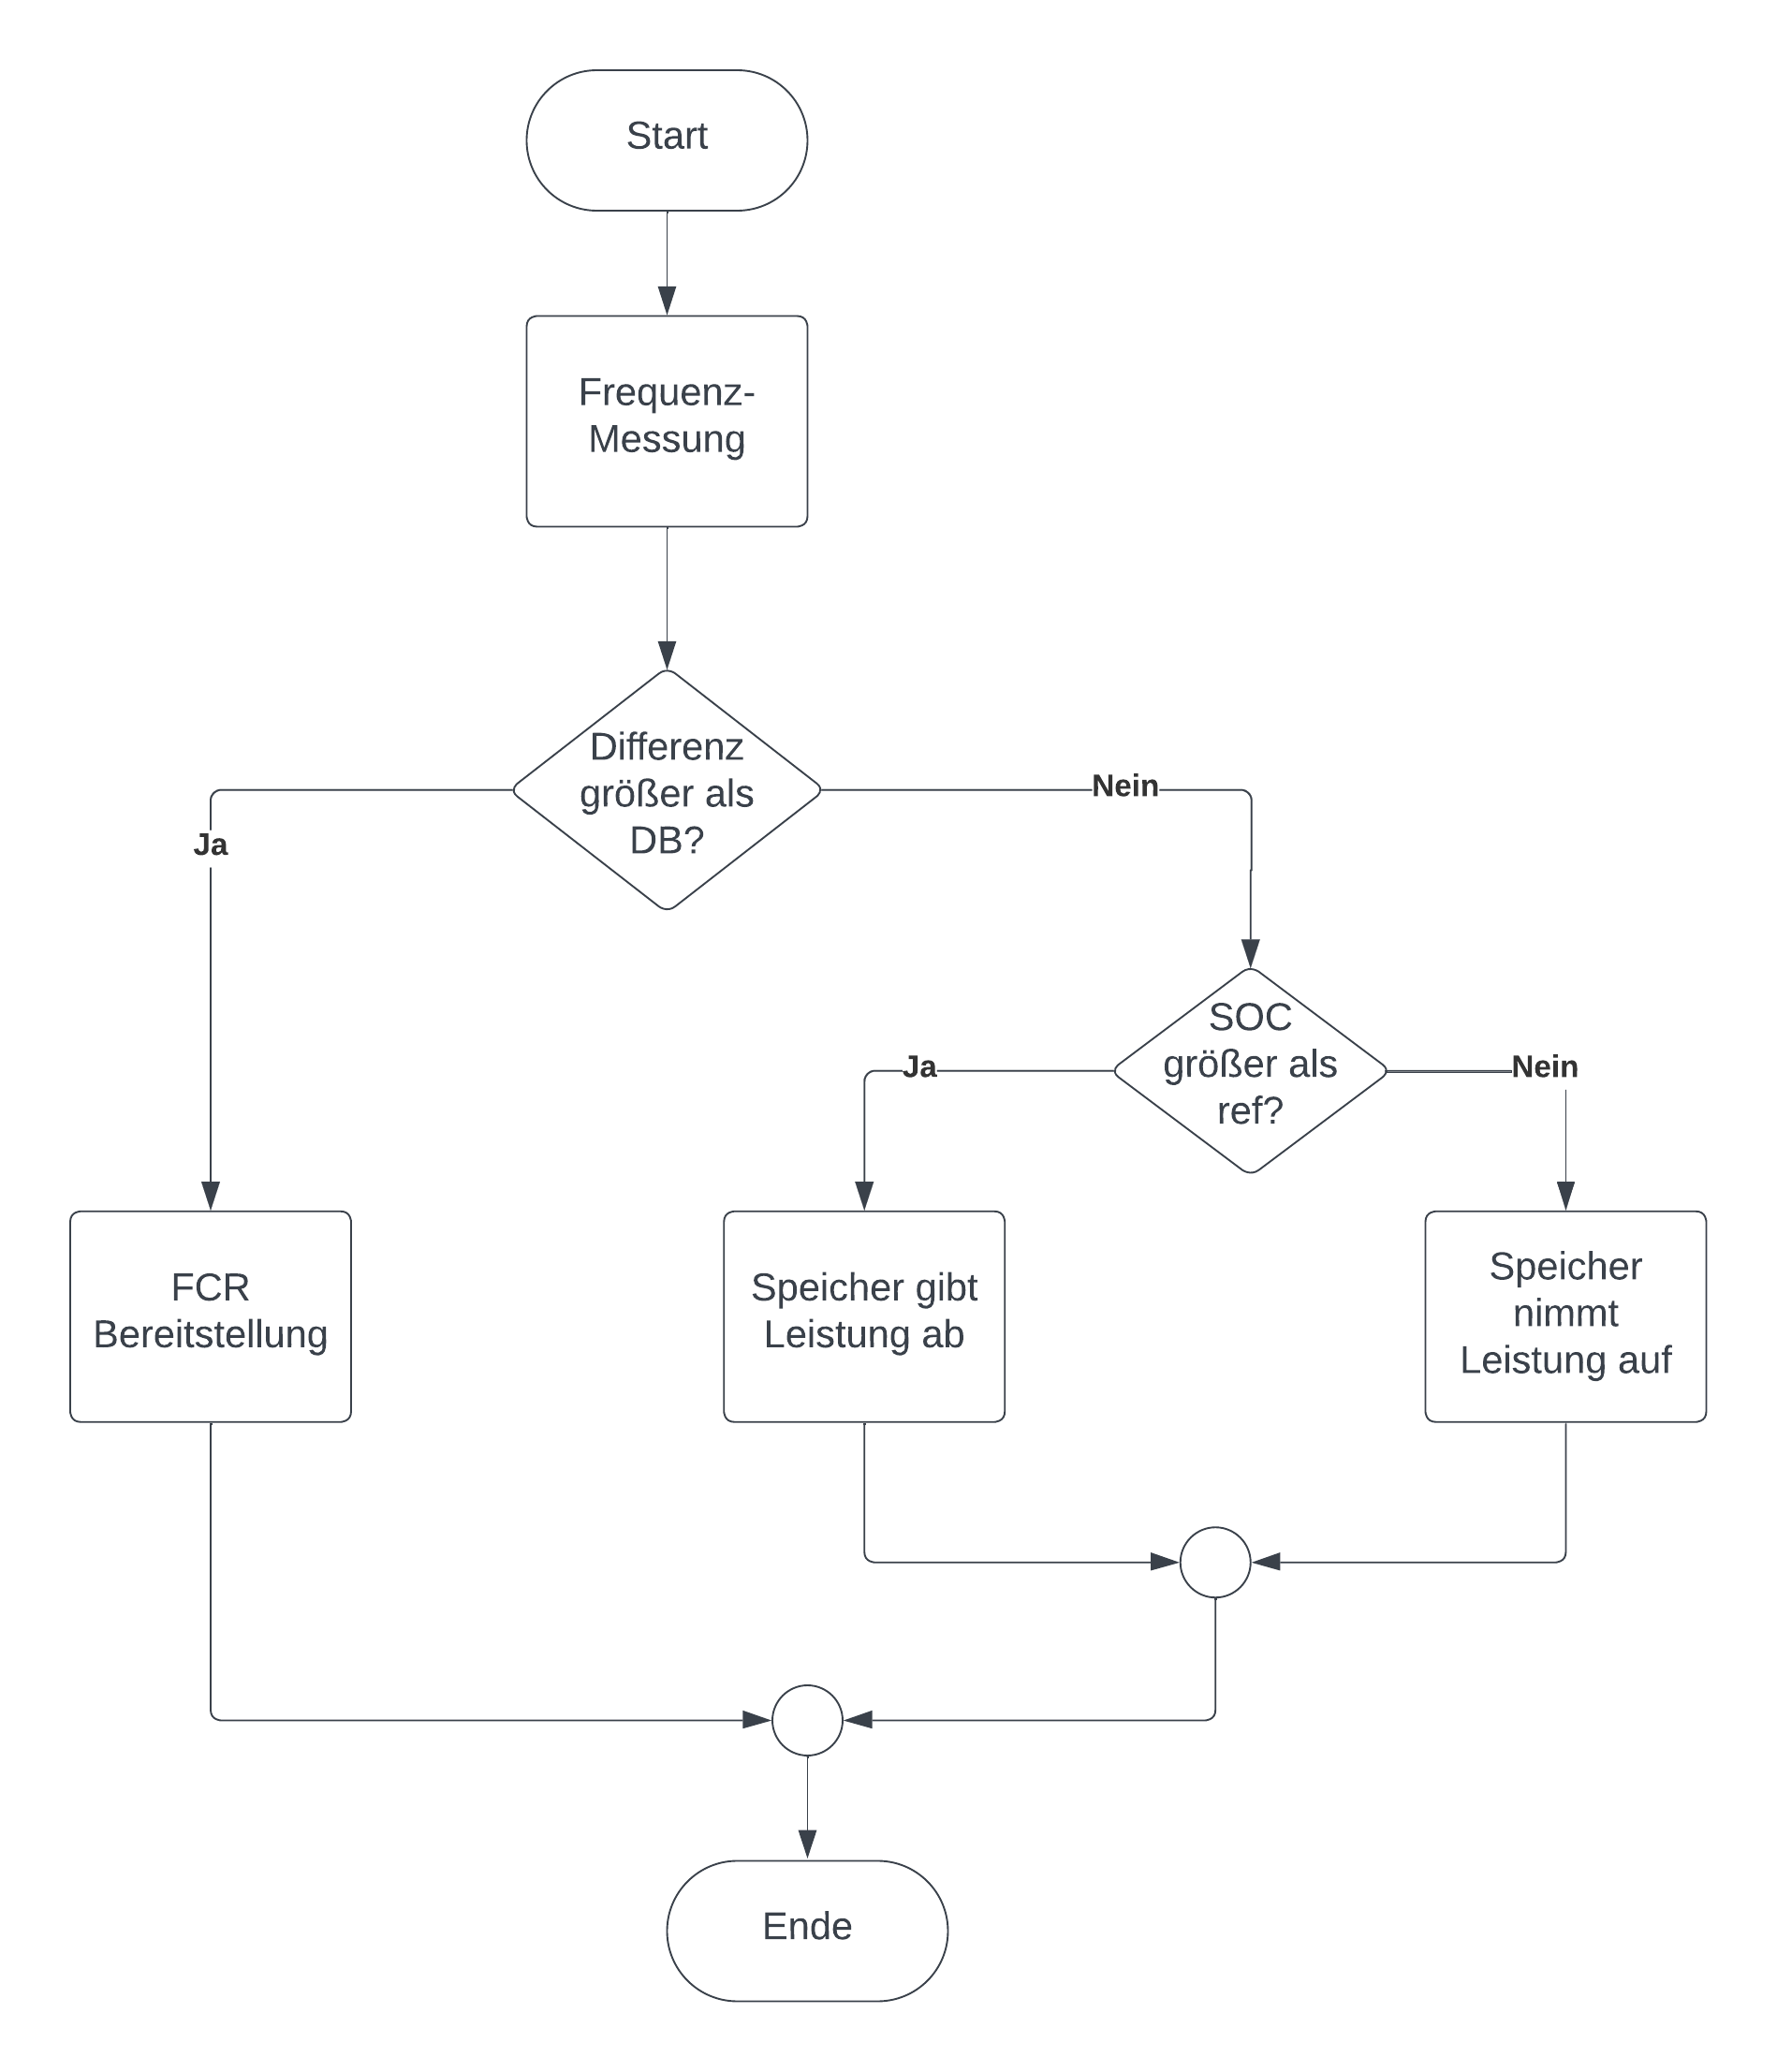
\includegraphics[width=8cm]{Abbildungen/DBFlow.png}
    \caption{Flussdiagramm zur Deadband-Strategie aus~\parencite[]{noauthor_soc_nodate}}\label{FlowPCR}
\end{figure}

Abbildung~\ref{FlowPCR} zeigt ein Flussdiagramm zur Ausnutzung des Totbands.
Ein Nachteil dieser Methode bleibt allerdings, dass nur bei geringen Abweichungen der Netzfrequenz und nur mit begrenzter 
Geschwindigkeit der Ziel-SOC hergestellt werden kann. 
Eine Überdimensionierung des Speichers, um auch bei längeren Störungen Regelleistung bereitstellen zu können, bleibt
also erforderlich.
Für das dreiphasige Modell dieser Projektarbeit soll diese Methode umgesetzt werden. 
Das Vorgehen dafür wird in Kapitel~\ref{Speicher} erläutert.

Ein weiterer Ansatz ist die Festlegung von Leistungssollwerten in Abhängigkeit vom aktuellen SOC.
Für dieses Vorgehen wird die Leistungskurve der Droop-Control um den Leistungssollwert $\Delta P_{SOC}$ nach oben
oder nach unten erweitert je nachdem ob der SOC unter oder über dem festgelegten Zielwert liegt.

\begin{figure}[h!]
    \centering
    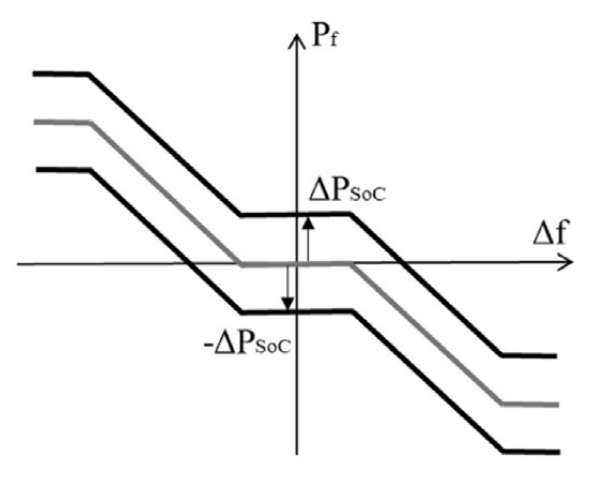
\includegraphics[width=7cm]{Abbildungen/DroopErweitert.png}
    \caption{SOC-Wiederherstellung mit Leistungssollwerten aus \parencite[]{noauthor_soc_nodate}}\label{Droopplus}
\end{figure}

Abbildung~\ref{Droopplus} zeigt den resultierenden Leistungsverlauf.
Dabei muss die maximale Leistungsaufnahme bzw. -abgabe der Batterie berücksichtigt werden und die Vorgaben der
Übertragungsnetzbetreiber müssen eingehalten werden.
Ein sehr ähnlicher Ansatz wird auch in \parencite[]{mantar_gundogdu_battery_2018} für den EFR-Einsatz genutzt.
Dort wird allerdings noch einmal hervorgehoben, dass ein starrer Ziel-SOC von z.B. exakt 50 \% die 
Anzahl der Lade- bzw. Entladezyklen erhöht und sich damit negativ auf die Lebensdauer der Batterien auswirkt.
Für die praktische Umsetzung sollte also ein SOC-Bereich von z.B. 45 \% bis 55 \% angestrebt werden.